\subsection{Seq2SeqLSTM}
La classe \texttt{Seq2SeqLSTM} implementa l'architettura specifica per il modello di summarization Sequence to Sequence con layer LSTM.\\
Vediamo di seguito le caratteristiche principali dell'architettura, composta da encoder e decoder:

\subsubsection{Encoder}
L'encoder è composto da:
\begin{itemize}
    \item \textbf{Layer di embedding}: mappa i token di input in vettori di lunghezza fissa
    \item \textbf{Tre layer LSTM} con:
        \begin{itemize}
            \item Dimensione latente fissa
            \item Dropout del 40\% 
            \item Recurrent dropout del 20\% 
        \end{itemize}
\end{itemize}

\subsubsection{Decoder}
Il decoder include:
\begin{itemize}
    \item \textbf{Layer di embedding}: mappa i token di output in vettori di lunghezza fissa
    \item \textbf{Layer LSTM} con:
        \begin{itemize}
            \item Stessa dimensione latente dell'encoder
            \item Dropout del 40\%
            \item Recurrent dropout del 20\%
        \end{itemize}
    \item \textbf{Layer di attention}: calcola i pesi di attenzione tra l'encoder e il decoder
    \item \textbf{Layer denso di output}: questo layer restituisce la distribuzione di probabilità sul vocabolario per la generazione delle parole del riassunto.\\ 
    Utilizza la funzione di attivazione softmax per la normalizzazione delle probabilità.
\end{itemize}

Di seguito, nella figura \ref{fig:seq2seqlstm_model_architecture}, possiamo vedere un diagramma dell'architettura del modello:

\begin{figure}[H]
    \centering
    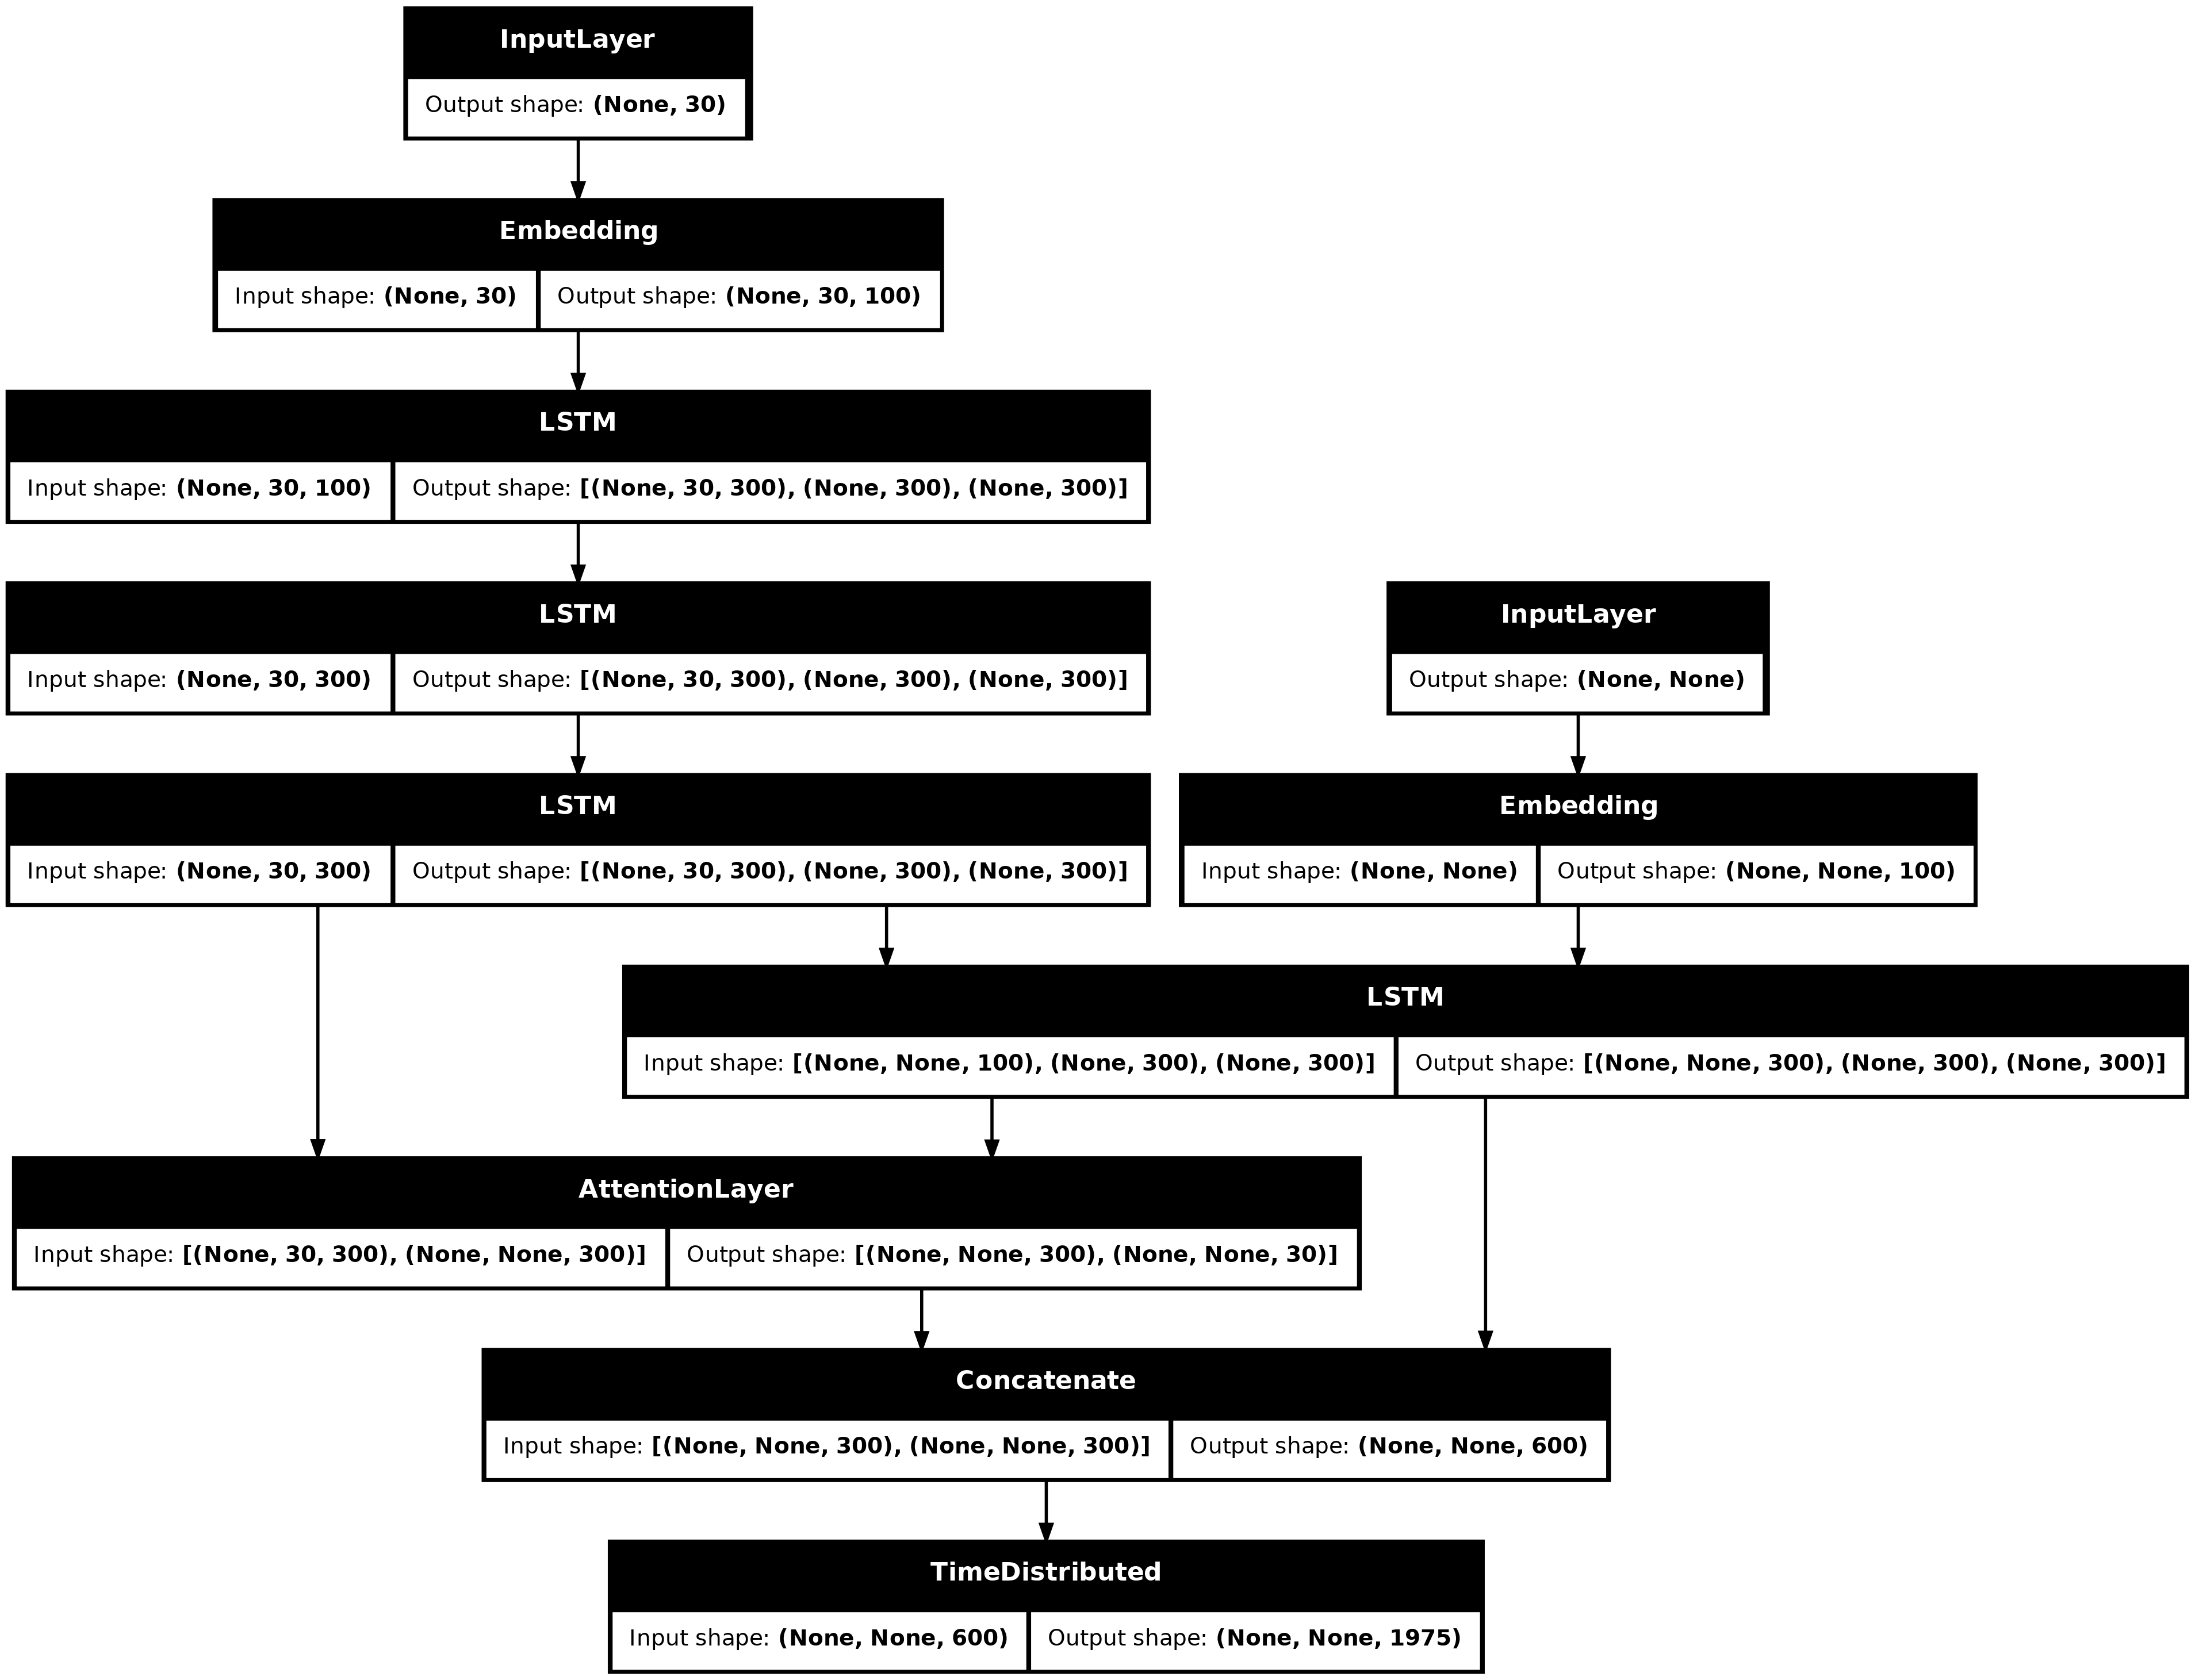
\includegraphics[width=1\textwidth]{media/Seq2SeqLSTM_originale_image.png}
    \caption{Diagramma dell'architettura del modello Seq2SeqLSTM}
    \label{fig:seq2seqlstm_model_architecture}
\end{figure}

\training{Adam}{50}
\risultati{DA INSERIRE}{DA INSERIRE}{DA INSERIRE}{DA INSERIRE}

Possiamo verifcare l'andamento delle loss durante l'addestramento nella figura \ref{fig:seq2seqlstm_loss_plot}.
\begin{figure}[H]
    \centering
    %TODO: Aggiungere immagine traingin loss È DA AGGIORNARE
    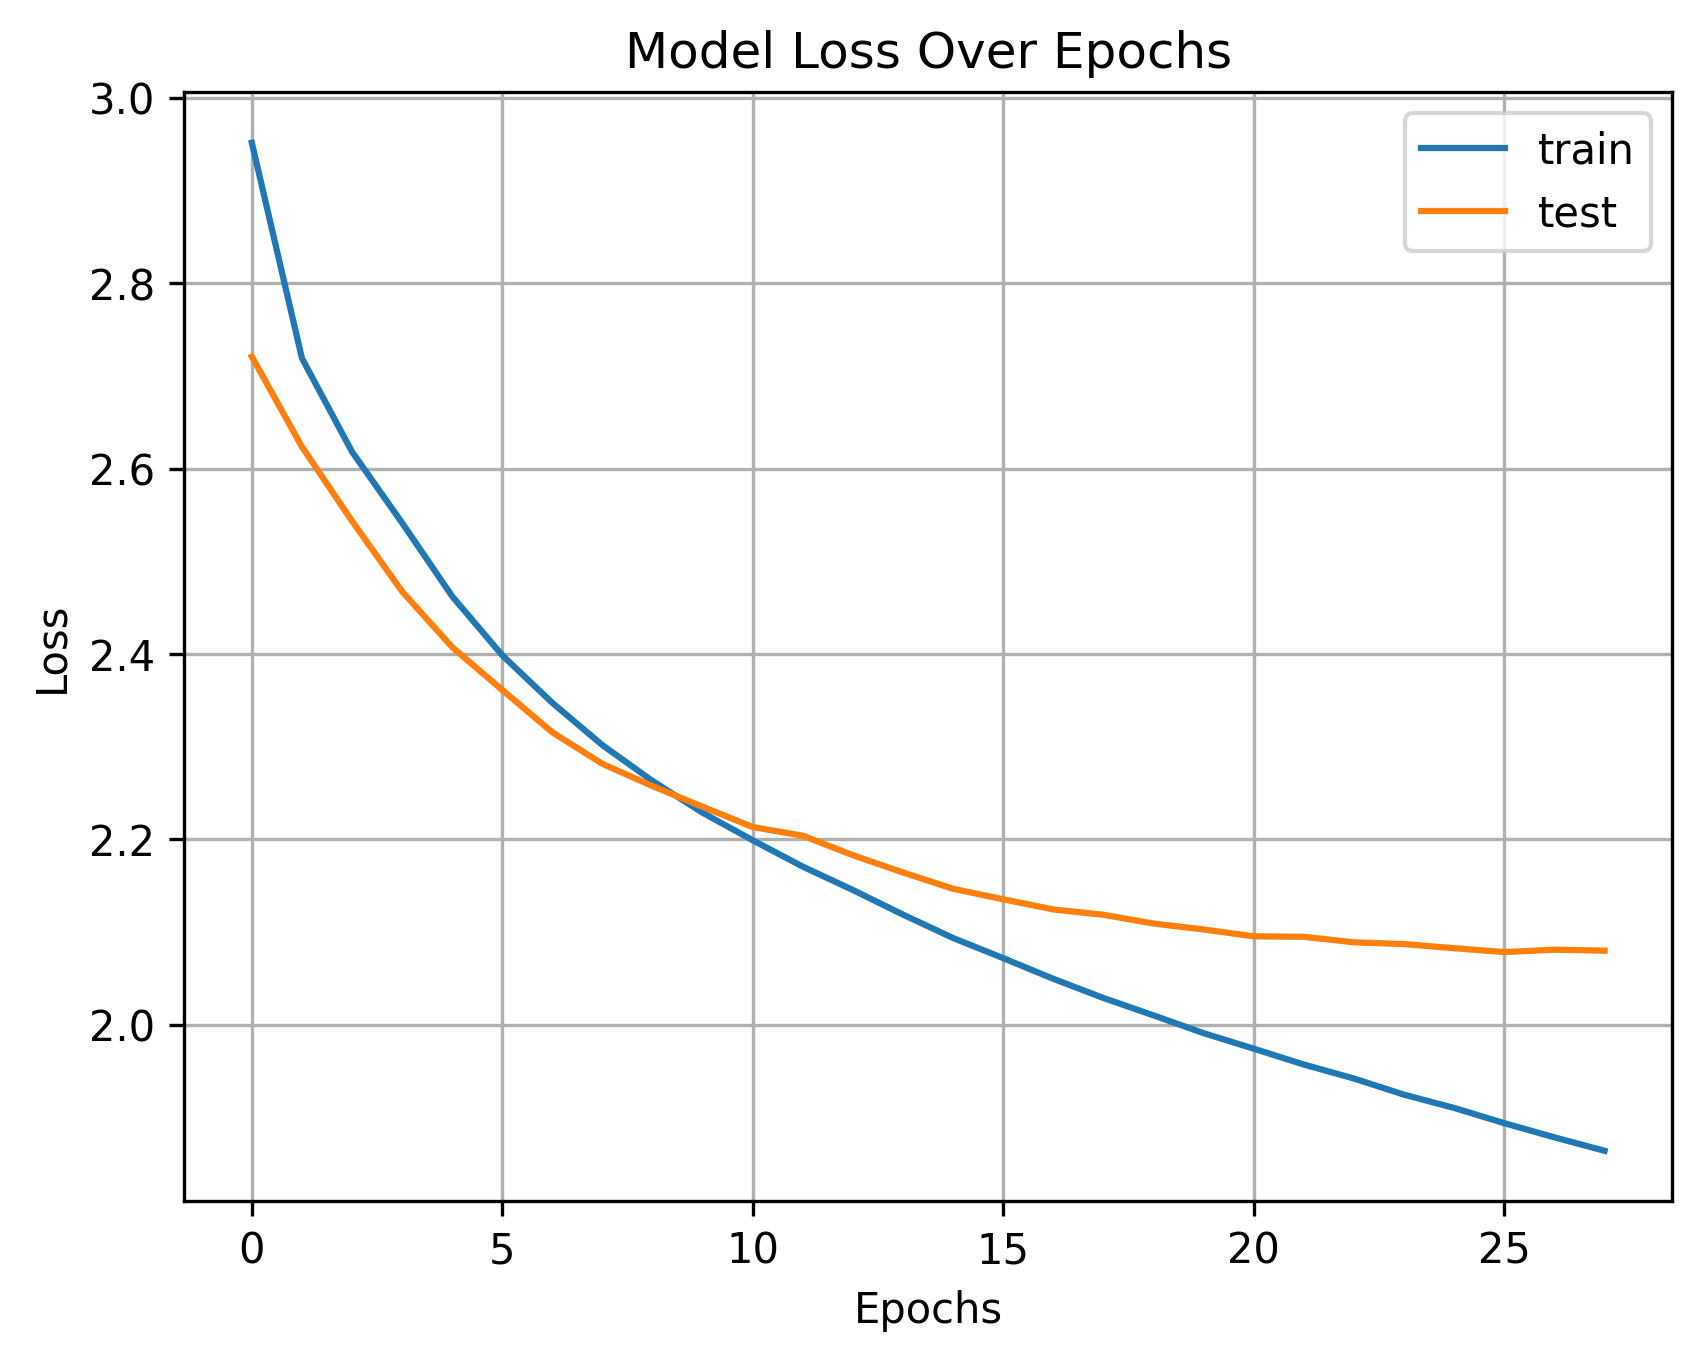
\includegraphics[width=0.75\textwidth]{media/Seq2SeqLSTM_originale_lossplot.png}
    \caption{Andamento delle loss durante l'addestramento}
    \label{fig:seq2seqlstm_loss_plot}
\end{figure}
